% ---------------------------------------------------------------
% Preamble
% ---------------------------------------------------------------
\documentclass[a4paper,11pt]{article}

\usepackage[utf8]{inputenc}
\usepackage[english]{babel}
\usepackage[margin=1in,a4paper,pdftex]{geometry}
\usepackage[protrusion=true,expansion=true]{microtype} 
\usepackage{amsmath,amsfonts,amsthm,amssymb,bm,mathdots,mathtools,bigints}
\usepackage{rotating}
\usepackage[colorlinks=true, linkcolor=blue, urlcolor=blue, anchorcolor=blue, citecolor=red]{hyperref}
\usepackage[all]{hypcap}
\usepackage{color, xcolor}
\usepackage{listings}
\usepackage[ruled,linesnumbered]{algorithm2e}
\usepackage{cite}
\usepackage{makecell}
\usepackage[printwatermark]{xwatermark}
\usepackage{subcaption}
\usepackage{siunitx}
\usepackage{tikz, pgfplots}

\usepackage{framed}
\definecolor{myYellow}{rgb}{1,0.65,0}
\definecolor{myRed}{rgb}{0.84, 0.18, 0.13}
\definecolor{myGreen}{rgb}{0, 0.53, 0.27}
\definecolor{myBlue}{rgb}{0, 0.34, 0.91}
\colorlet{shadecolor}{myBlue!7}

\numberwithin{figure}{section}
\numberwithin{equation}{section}
\numberwithin{table}{section}

\newtheorem{theorem}{Theorem}[section]
\newtheorem{corollary}{Corollary}[theorem]
\newtheorem{lemma}[theorem]{Lemma}

\theoremstyle{definition}
\newtheorem{definition}{Definition}[section]

%\newwatermark[allpages,color=red!15,angle=45,scale=5,xpos=-1cm,ypos=2cm]{DRAFT}

\makeatletter
\setlength{\@fptop}{0pt}
\makeatother

\usepackage{graphicx}
\graphicspath{ {figs/} }

\newbox{\bigpicturebox}

\lstset{
    backgroundcolor=\color[rgb]{0.86,0.88,0.93},
    language=matlab, keywordstyle=\color[rgb]{0,0,1},
    basicstyle=\footnotesize \ttfamily,breaklines=true,
    escapeinside={\%*}{*)}
}

% --------------------------------------------------------------------
% Tikz Macros
% --------------------------------------------------------------------
\usetikzlibrary{shapes,arrows, backgrounds, positioning, fit, decorations.pathmorphing}

\tikzstyle{sectionBlock} = [draw, fill=blue!20, rectangle, minimum height=3em, minimum width=3em]
\tikzstyle{block} = [draw, fill=white, rectangle, minimum height=3em, minimum width=3em]
\tikzstyle{sum} = [draw, fill=white, circle, node distance=1cm]
\tikzstyle{input} = [coordinate]
\tikzstyle{output} = [coordinate]
\tikzstyle{pinstyle} = [pin edge={to-,thin,black}]
\tikzstyle{mcInput} = [draw, rectangle, line width=0.5mm, minimum width=2em, minimum height=2em, fill=black!10]
\tikzstyle{mcCircle} = [draw, circle, line width=0.5mm, minimum width=2em, minimum height=2em, fill=white]

% --------------------------------------------------------------------
% Definitions
% --------------------------------------------------------------------
\newcommand{\HRule}[1]{\rule{\linewidth}{#1}} 

\makeatletter                       
\def\printtitle{
    {\centering \@title\par}}
\makeatother                                    

\makeatletter 
\def\printauthor{
    {\centering \large \@author}}               
\makeatother                            

\newcounter{boxed-theorem}
\makeatletter
\newenvironment{boxed-theorem}[1]
{\begin{shaded} \begin{theorem}{#1}}
{\end{theorem} \end{shaded}}

\newcounter{boxed-definition}
\makeatletter
\newenvironment{boxed-definition}[1]
{\begin{shaded} \begin{definition}{#1}}
{\end{definition} \end{shaded}}

% ---------------------------------------------------------------
% Metadata 
% ---------------------------------------------------------------
\title{ \normalsize \textsc{TI0119 - PROCESSAMENTO DIGITAL DE SINAIS} 
        \\[2.0cm]             
        \HRule{0.5pt} \\              
        \LARGE \textbf{\uppercase{Transformada Z}\\1º Exerc\'icio Computacional}
        \HRule{2pt} \\[0.5cm]  
}

\author{
        Otacílio Bezerra Leite Neto\\   
        Universidade Federal do Ceará\\  
        Departamento de Engenharia de Teleinform\'atica\\
        \texttt{minhotmog@gmail.com} \\
}

\begin{document}
% ---------------------------------------------------------------
% Maketitle
% ---------------------------------------------------------------
\thispagestyle{empty}       % Remove page numbering on this page

\printtitle                 % Print the title data as defined above
    \vfill
\printauthor                % Print the author data as defined above
\newpage

% ---------------------------------------------------------------
% Begin document
% ---------------------------------------------------------------

% 1 - Introduction
% ---------------------------------------------------------------
\clearpage
\setcounter{page}{1}
\section{Sinal de Filtro de 1a Ordem}

No primeiro exemplo, iremos visualizar os polos e zeros, no Plano Z, e os gr\'aficos de magnitude e fase do seguinte sistema:
\begin{equation} \label{eq:first-system}
	H(z) = \cfrac{1}{1-a z^{-1}}
\end{equation}

O resultado para diferentes valores de $a$ entre $[-1.5, 1.5]$ s\~ao demonstrados na Fig. \ref{fig:01}, onde cada cor relaciona um polo no Plano Z a um par de curvas de magnitude e fase.

\begin{figure}[ht]
	\centering
	\begin{subfigure}{0.49\textwidth}
		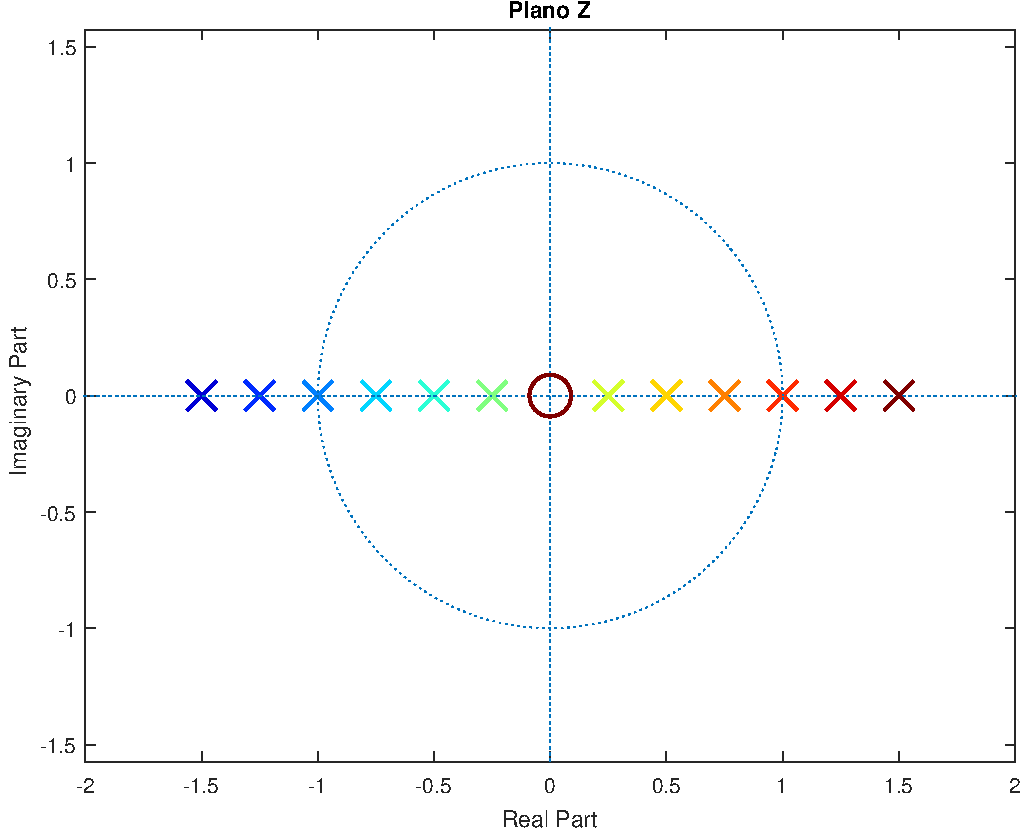
\includegraphics[width=\textwidth]{ex_1_pz}
	\end{subfigure}
	\begin{subfigure}{0.49\textwidth}
		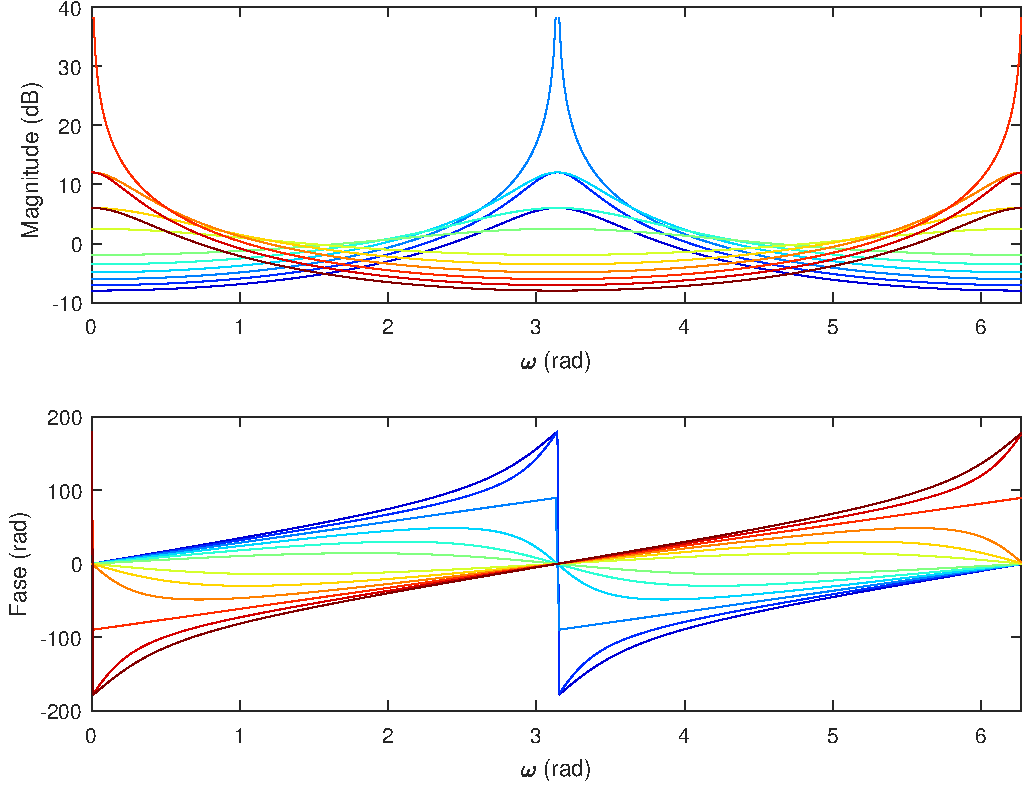
\includegraphics[width=\textwidth]{ex_1_bode}
	\end{subfigure}
		
	\caption{Visualizaç\~ao do Plano Z e das componentes de magnitude e fase para \eqref{eq:first-system}}
	\label{fig:01}
\end{figure}

Pelas visualizaç\~oes podemos notar uma relaç\~ao entre a posiç\~ao dos polos no plano complexo com as componentes de magnitude e fase do sinal resultante. Primeiramente, note que o valor do pico da magnitude tende a crescer \`a medida que fazemos os polos se aproximarem do c\'irculo de raio unit\'ario (centrado na origem). Nesse caso, os maiores picos se encontram na frequ\^encia $\omega = \pi$, quando o polo $a = -1$, e nas frequ\^encias $\omega = 0$ e $\omega= 2\pi$, quando o polo $a = 1$. Para entender o porqu\^e dessa ocorr\^encia, primeiro note que, pela \'algebra complexa, a magnitude da resposta de um sistema pode ser calculada como:
\begin{equation}
	| H(z) | = \cfrac{| N(z) |}{| D(z) |} = \cfrac{| 1 |}{| 1 - az^{-1} |} 
\end{equation}

\noindent onde o denominador resultante \'e interpretado como a dist\^ancia no plano Z de um ponto qualquer at\'e o polo $a$. Nesse caso, se avaliarmos a magnitude do sinal quando $a = -1$, para um ponto no raio unit\'ario dado como $z = 0-j1$, veremos que um valor nulo surgir\'a no denominador. Como resultado, a magnitude calculada aproxima-se ao infinito quando o polo se aproxima do circulo de raio unit\'ario. Perceba que o mesmo racioc\'inio \'e v\'alido para o polo $a = 1$, quando avaliado sobre $z = 0+1j$.

Utilizando \'algebra complexa, tamb\'em \'e poss\'ivel caracterizar a f\'ormula da fase:
\begin{equation}
	\angle H(e^{j\omega}) = \sum_{k=0}^M \angle (1 - n_k e^{-jw}) - \sum_{k=0}^M \angle (1 - d_k e^{-jw}) = - \angle (1 - a e^{-jw})
\end{equation}

\noindent onde $n_k$ e $d_k$ s\~ao, respectivamente, um zero e um polo do sistema. Note que, com essa f\'ormula, \'e poss\'ivel interpretar a fase resultante como a diferença do \^angulo de um vetor que parte do zero at\'e um ponto no c\'irculo unit\'ario com o \^angulo de um vetor que parte do polo at\'e esse mesmo ponto. Por esse exato motivo \'e poss\'ivel entender porque a fase do sistema sofre uma invers\~ao mais acentuada na frequ\^encia $\omega = \pi$ quando os polos est\~ao localizados no lado esquerdo do plano, enquanto que sofre uma invers\~ao mais acentuada nas frequ\^encias $\omega = 0$ e $\omega = 2\pi$ quando os polos est\~ao localizados no lado direito.


\section{Sinal de Filtro de Ordem N}

No segundo exemplo, iremos visualizar os polos e zeros, no Plano Z, e os gr\'aficos de magnitude e fase do seguinte sistema:
\begin{equation} \label{eq:second-system}
	H(z) = \cfrac{1 - a^nz^{-n}}{1-a z^{-1}} = 1 - a^{n-1}z^{-(n-1)}
\end{equation}

Antes de mais nada, note que para este espec\'ifico exemplo foi poss\'ivel realizar o \textit{Cancelamento de Polos e Zeros} para simplificar a funç\~ao de trasnfer\^encia ao remover o polo em $z = a + j0$ com o zero existente nessa posiç\~ao. O resultado para diferentes valores pares de $n$ entre $[4, 10]$ s\~ao demonstrados na Fig. \ref{fig:02}, para diferentes valores de $a$ entre $[0.2, 0.8]$, e na Fig. \ref{fig:03}, para diferentes valores positivos de $a$ entre $[-0.8, -0.2]$, onde cada cor relaciona um zero no Plano Z a um par de curvas de magnitude e fase.

Pela visualizaç\~ao, o primeiro padr\~ao que torna-se evidente consiste na relaç\~ao do n\'umero de zeros no plano complexo com o n\'umero de componentes de frequ\^encia nas magnitudes e fases do sistema. De fato, como um c\'irculo no Plano Z est\'a relacionado a um valor de frequ\^encia, o n\'umero de zeros em um mesmo c\'irculo diretamente indica o n\'umero de oscilaç\~oes que a magnitude e a fase realizam em uma revoluç\~ao completa de $2\pi$. A dist\^ancia dos zeros para o centro do plano (e, consequentemente, aos zeros do sistema) providenciam a informaç\~ao da magnitude dos picos do sinal. Esse fato se torna ainda mais evidente se analisarmos a f\'ormula de Euler para o n\'umero complexo $z$ na equaç\~ao \eqref{eq:second-system}:
\begin{equation} \label{eq:third-system}
	H(z) = 1 - a^{n-1}z^{-(n-1)} = 1 - a^{n-1} r^{-(n-1)} \left( cos[(n-1) \omega] - j sen[(n-1) \omega] \right)
\end{equation}

\noindent onde $r^{-(n-1)}$ representa a amplitude do n\'umero complexo $z^{-(n-1)}$. Perceba, ent\~ao, que um aumento do valor de $n$ est\'a diretamente relacionado \`a frequ\^encia das componentes oscilat\'orias do sinal.

Note que, no que cerne ao pico das magnitudes, todas as visualizaç\~oes seguiram o mesmo resultado discutido anteriormente, onde nesse caso os picos se localizam nas frequencias $\omega = 0$ e $\omega = 2\pi$ quando apenas valores positivos de $a$ se aproximam do c\'irculo unit\'ario, enquanto que os picos se localizam nas frequ\^encias $\omega = \pi$ no caso dos valores negativos de $a$, como demonstrado respectivamente nas duas figuras.

\begin{figure}[ht]
	\centering
	\begin{subfigure}{0.44\textwidth}
		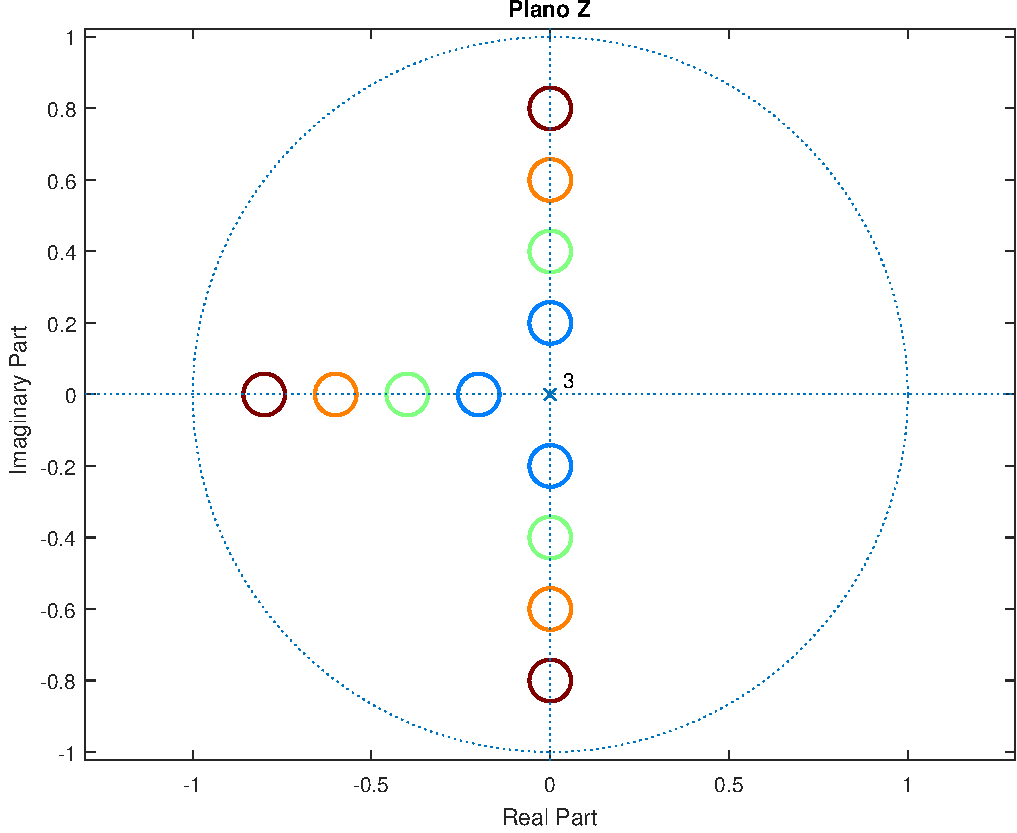
\includegraphics[width=\textwidth]{ex_2_pz_4}
	\end{subfigure}
	\begin{subfigure}{0.44\textwidth}
		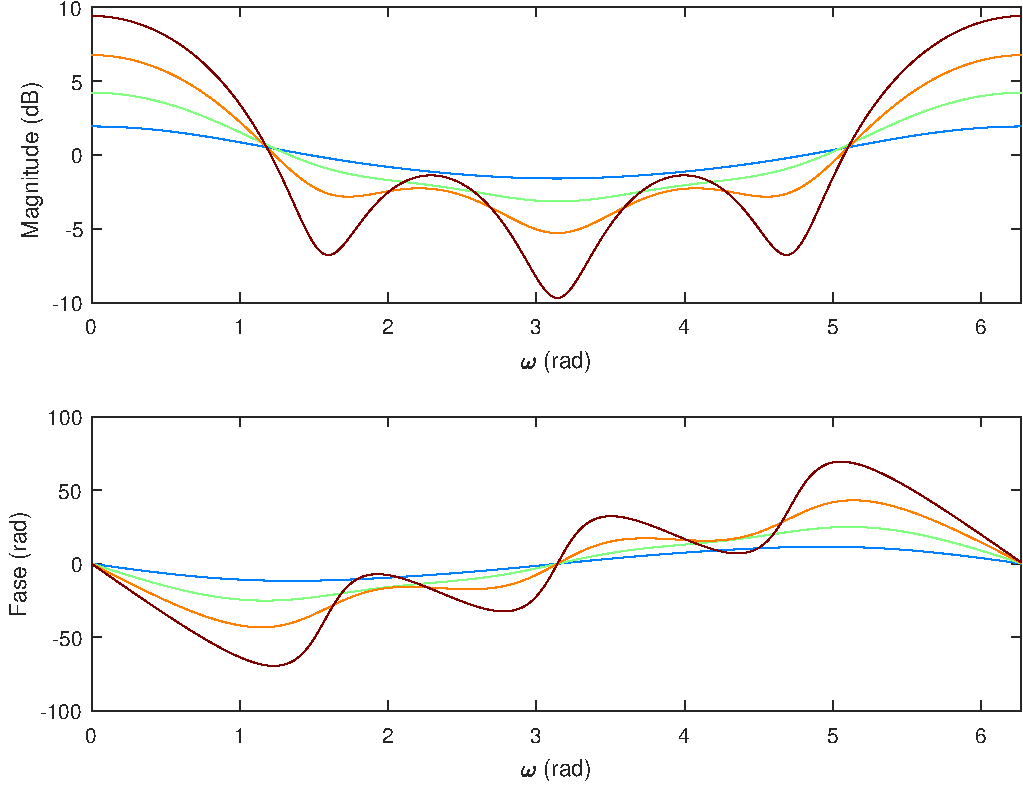
\includegraphics[width=\textwidth]{ex_2_bode_4}
	\end{subfigure}\\
	\begin{subfigure}{0.44\textwidth}
		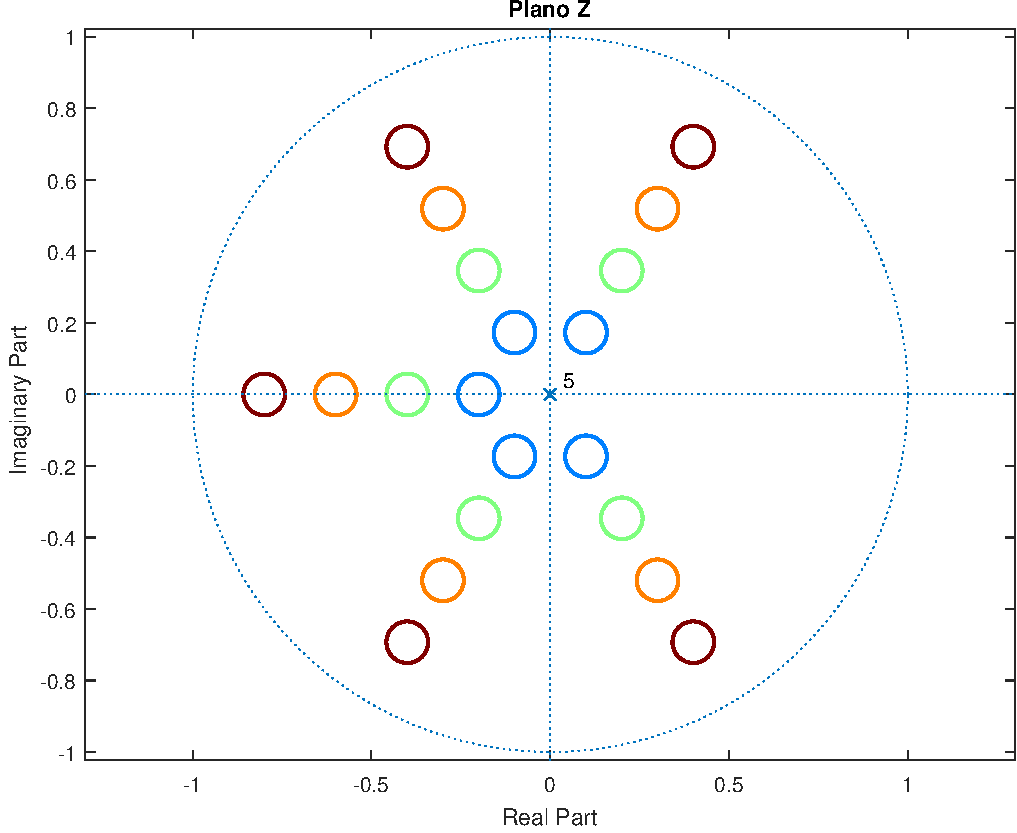
\includegraphics[width=\textwidth]{ex_2_pz_6}
	\end{subfigure}
	\begin{subfigure}{0.44\textwidth}
		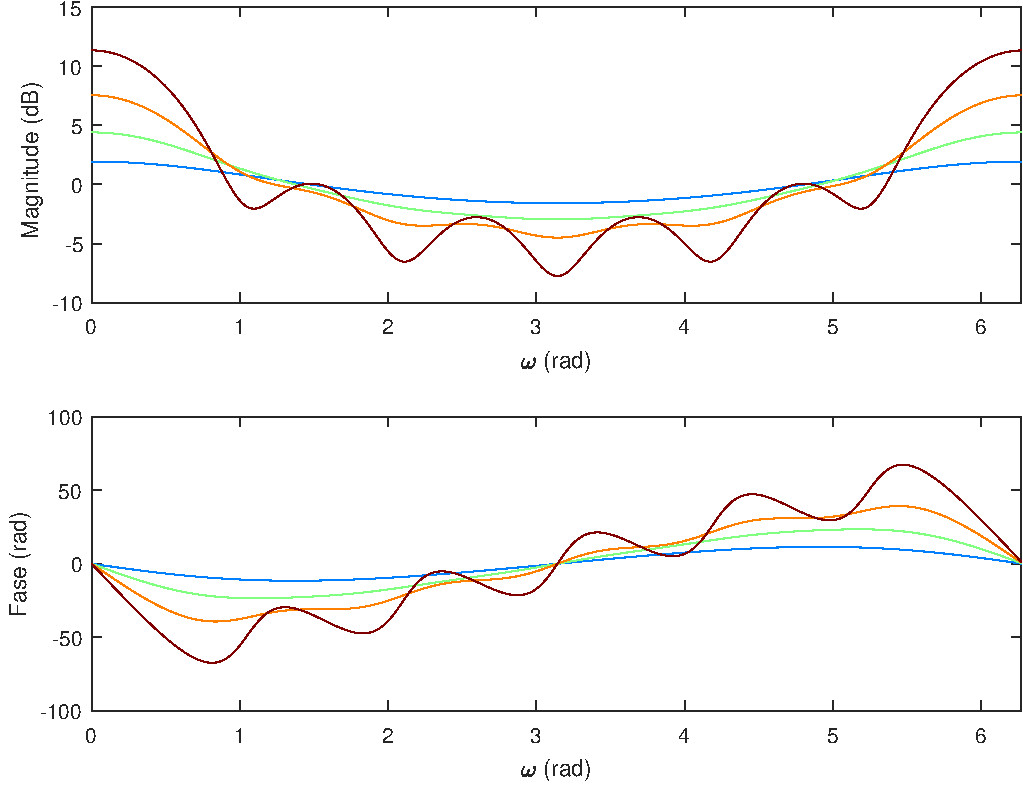
\includegraphics[width=\textwidth]{ex_2_bode_6}
	\end{subfigure}\\
	\begin{subfigure}{0.44\textwidth}
		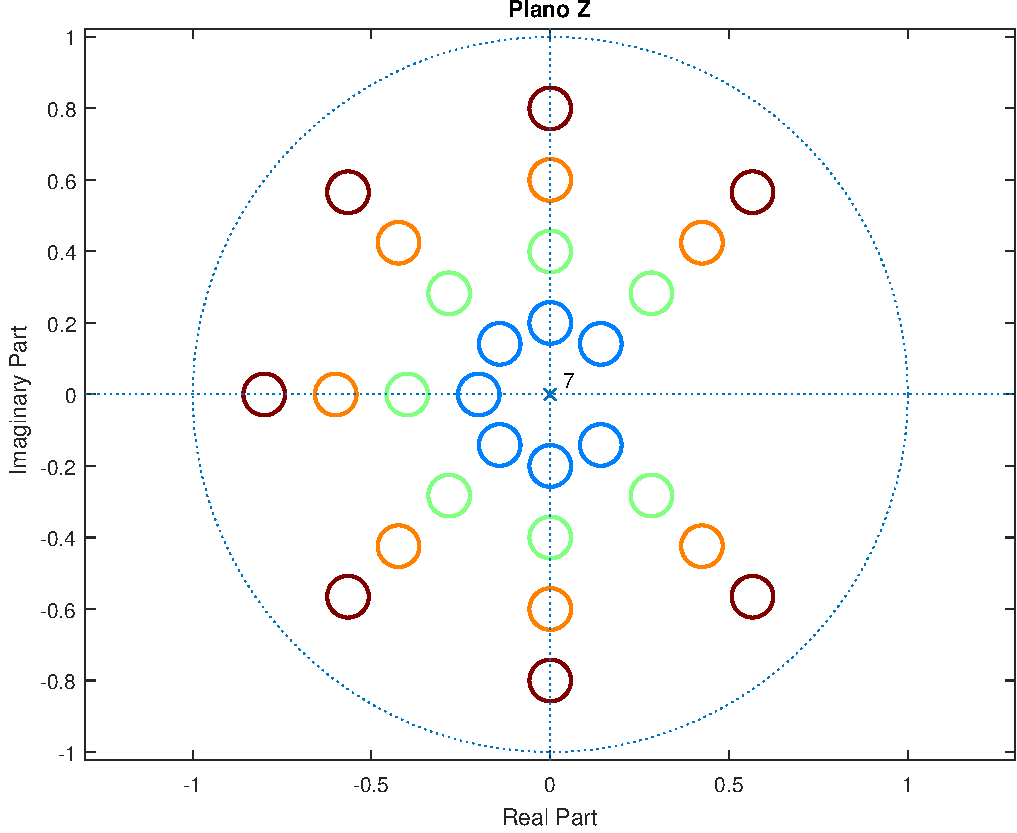
\includegraphics[width=\textwidth]{ex_2_pz_8}
	\end{subfigure}
	\begin{subfigure}{0.44\textwidth}
		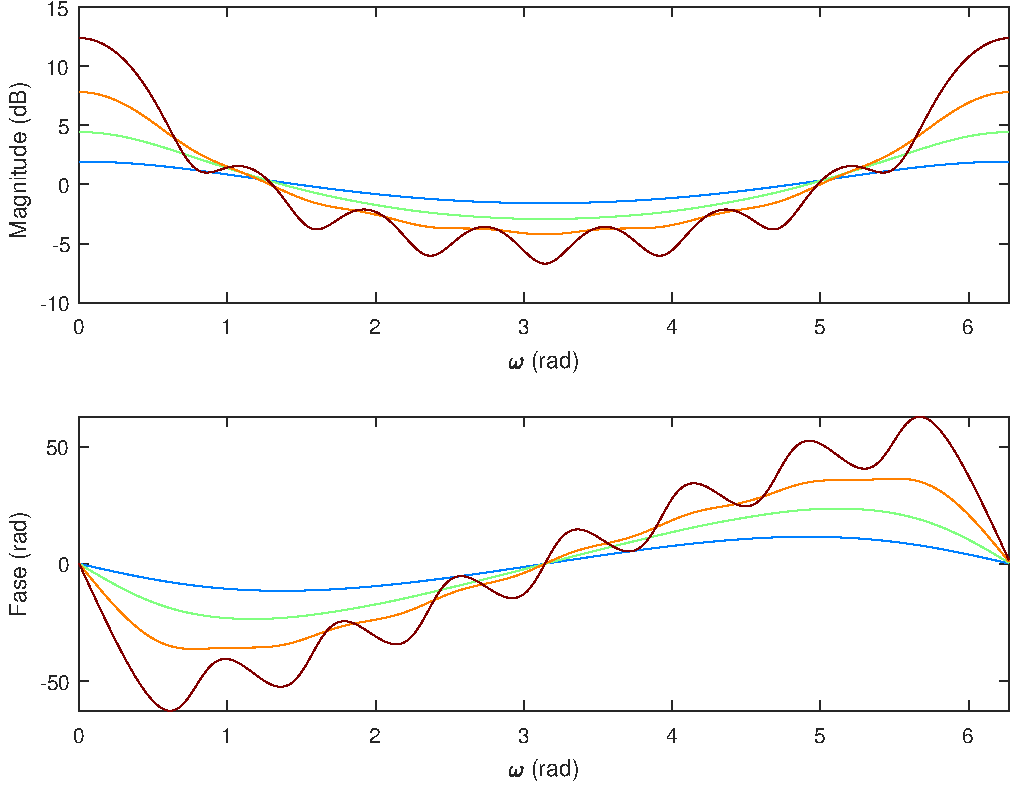
\includegraphics[width=\textwidth]{ex_2_bode_8}
	\end{subfigure}\\
	\begin{subfigure}{0.44\textwidth}
		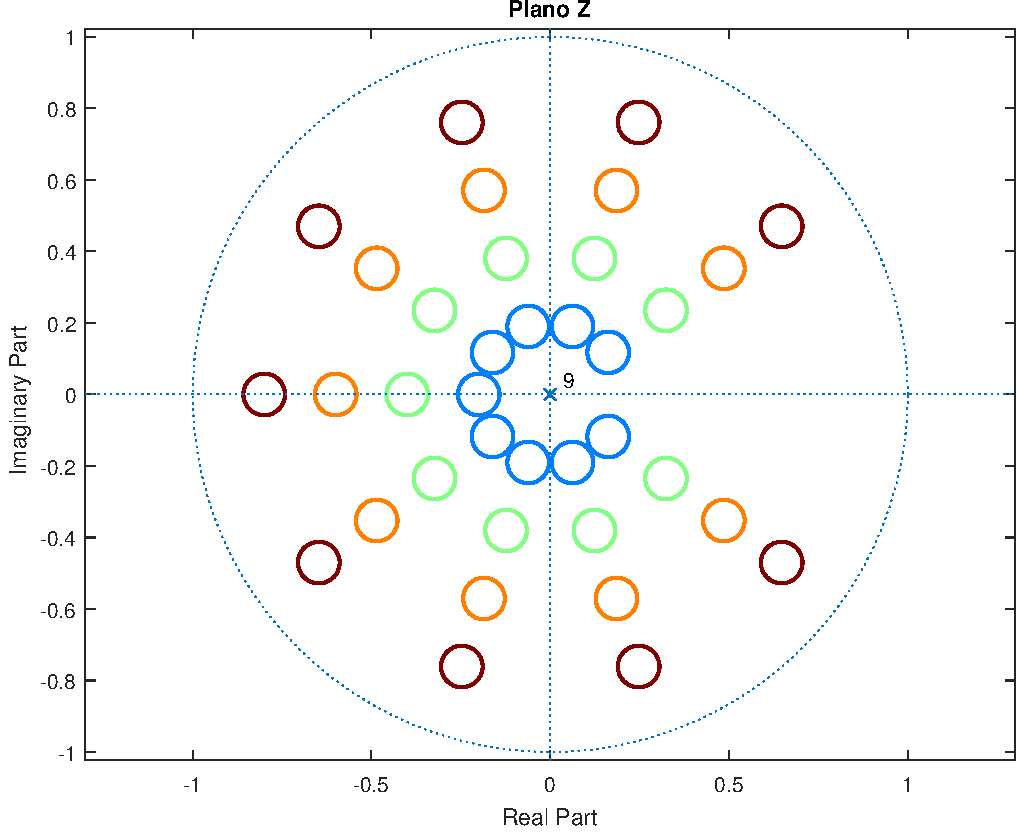
\includegraphics[width=\textwidth]{ex_2_pz_10}
	\end{subfigure}
	\begin{subfigure}{0.44\textwidth}
		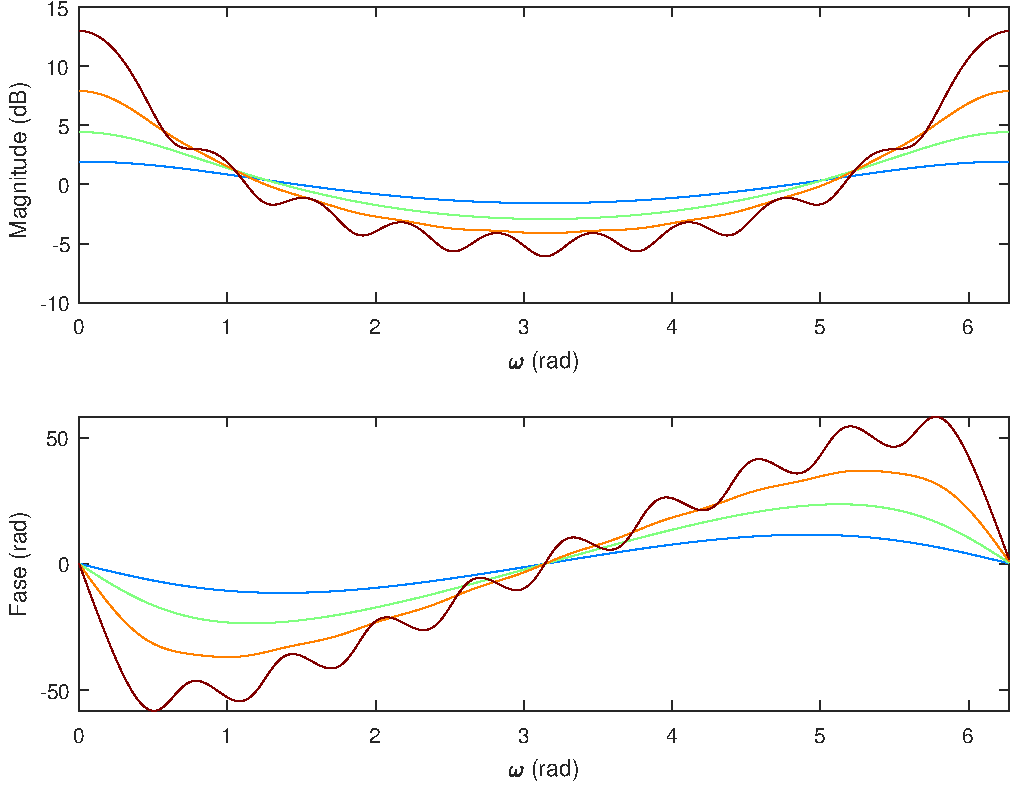
\includegraphics[width=\textwidth]{ex_2_bode_10}
	\end{subfigure}\\
		
	\caption{Visualizaç\~ao do Plano Z e das componentes de magnitude e fase para o sistema em \eqref{eq:second-system} com o par\^ametro $a > 0$}
	\label{fig:02}
\end{figure}

\begin{figure}[ht]
	\centering
	\begin{subfigure}{0.44\textwidth}
		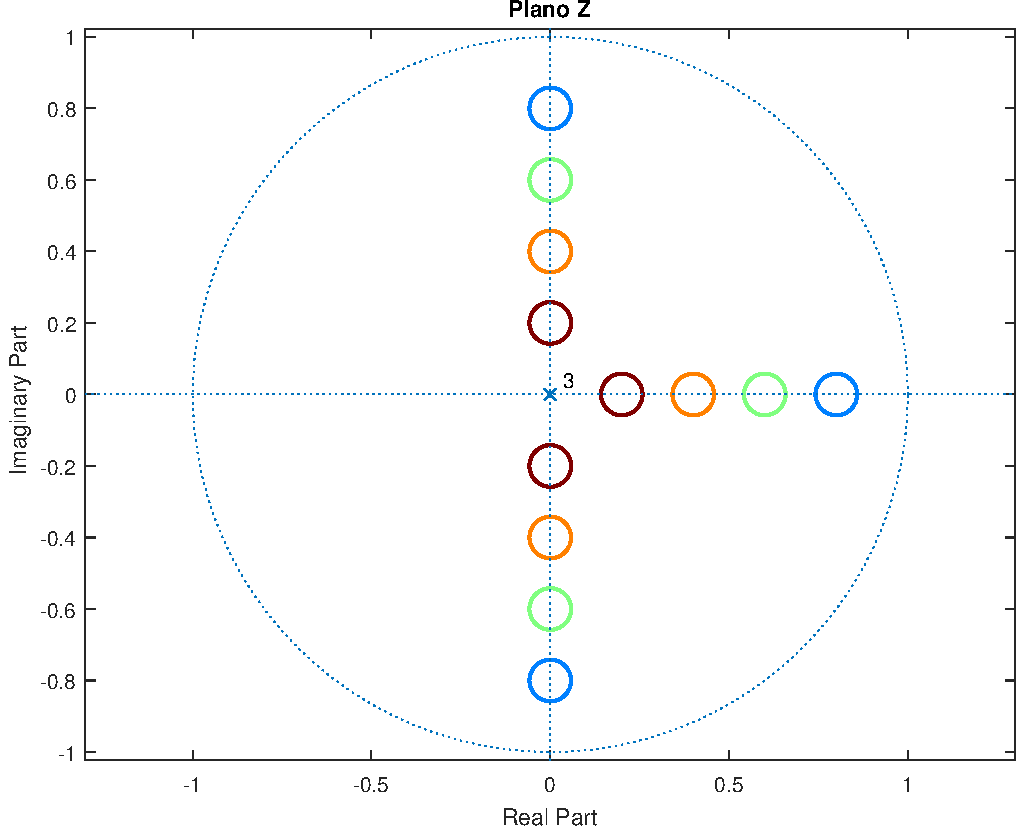
\includegraphics[width=\textwidth]{ex_3_pz_4}
	\end{subfigure}
	\begin{subfigure}{0.44\textwidth}
		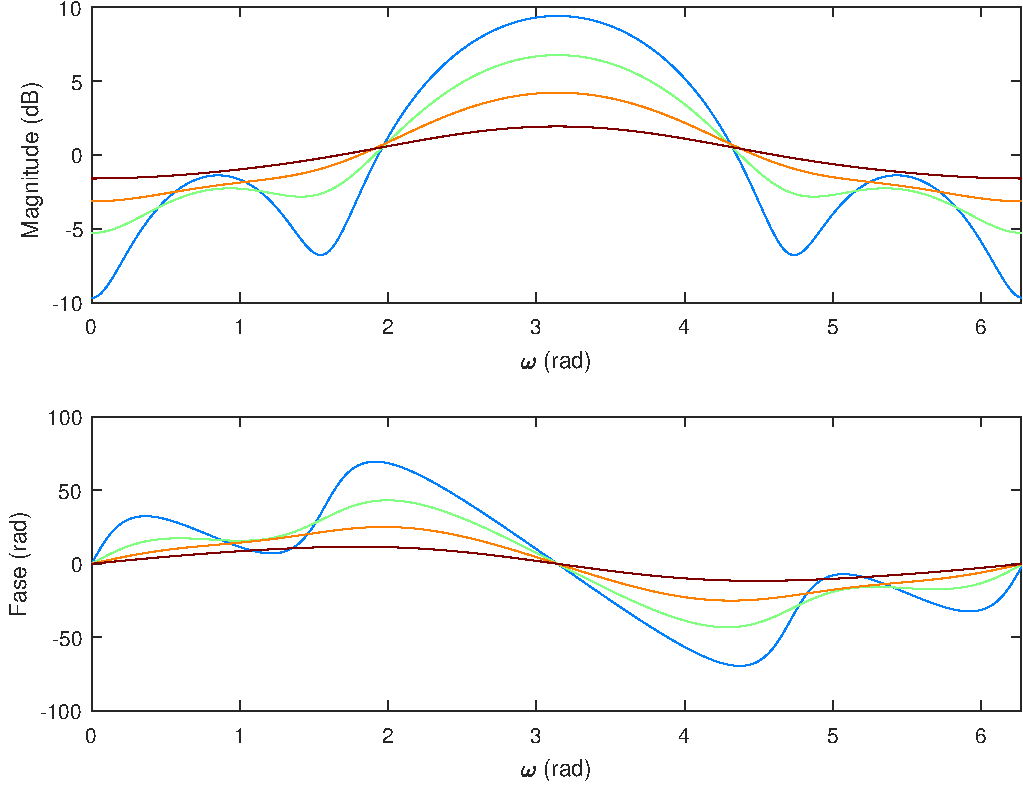
\includegraphics[width=\textwidth]{ex_3_bode_4}
	\end{subfigure}\\
	\begin{subfigure}{0.44\textwidth}
		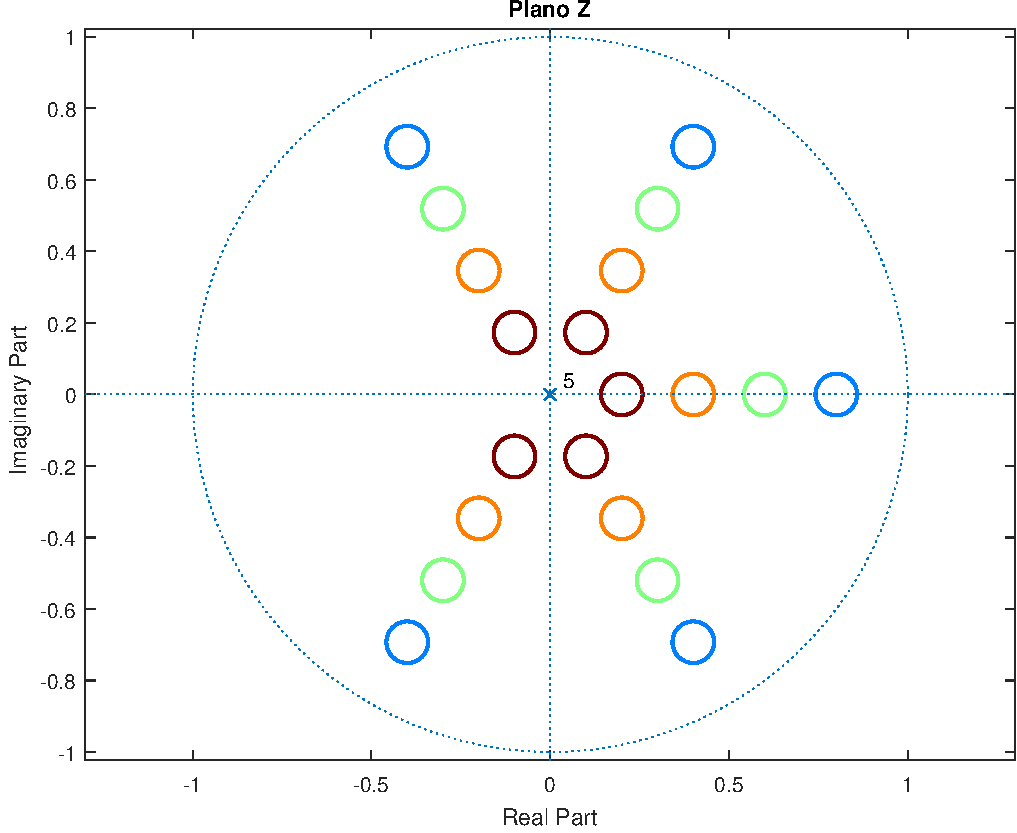
\includegraphics[width=\textwidth]{ex_3_pz_6}
	\end{subfigure}
	\begin{subfigure}{0.44\textwidth}
		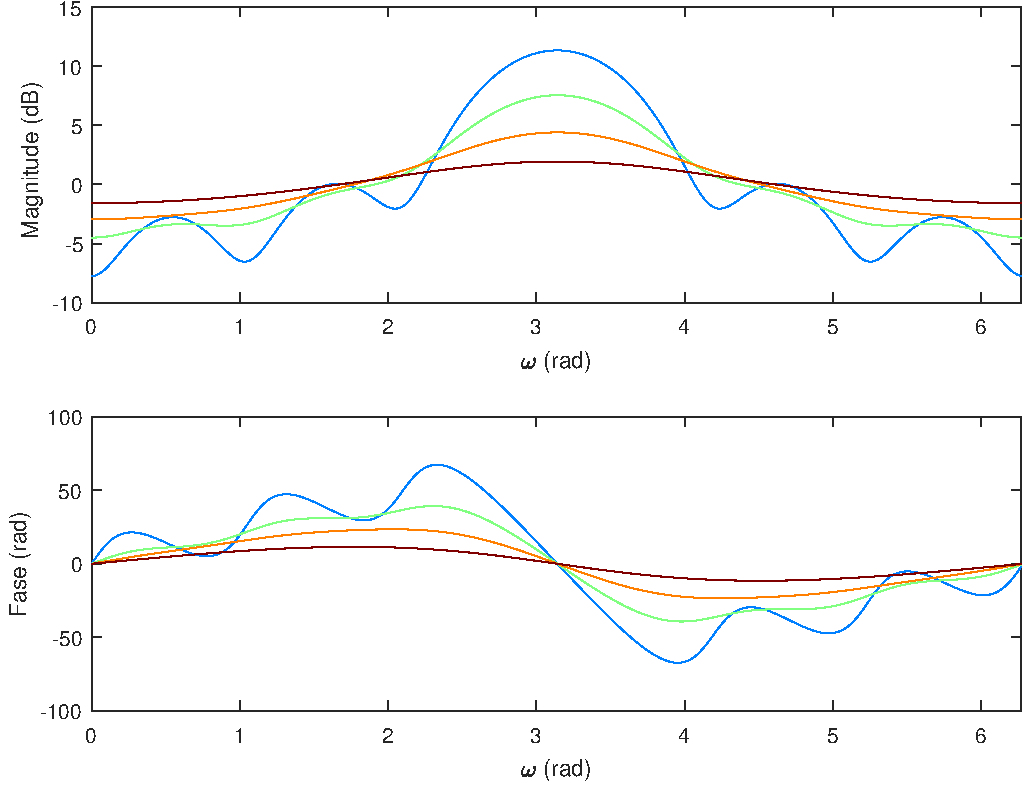
\includegraphics[width=\textwidth]{ex_3_bode_6}
	\end{subfigure}\\
	\begin{subfigure}{0.44\textwidth}
		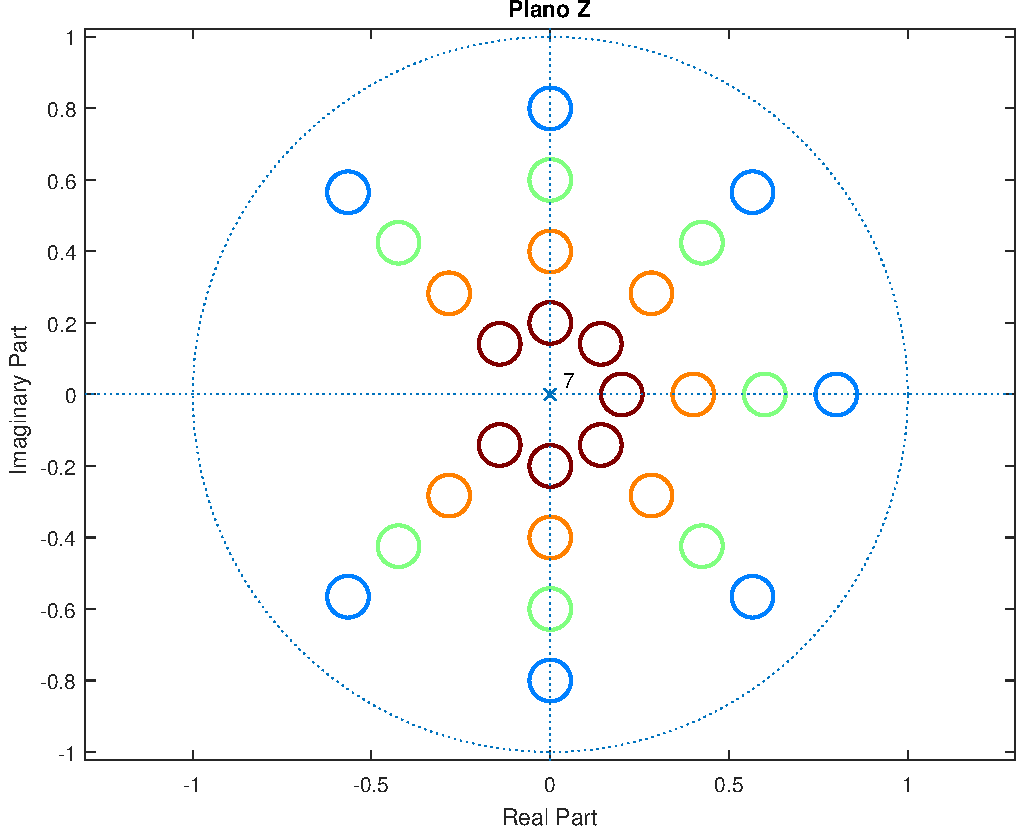
\includegraphics[width=\textwidth]{ex_3_pz_8}
	\end{subfigure}
	\begin{subfigure}{0.44\textwidth}
		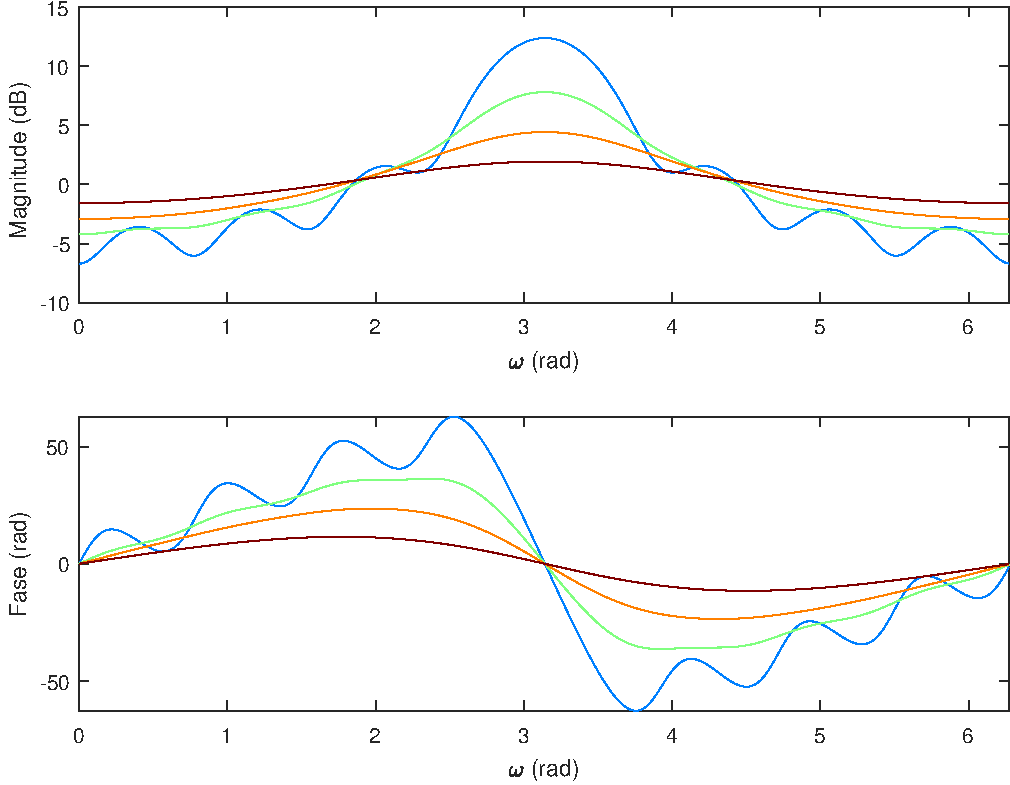
\includegraphics[width=\textwidth]{ex_3_bode_8}
	\end{subfigure}\\
	\begin{subfigure}{0.44\textwidth}
		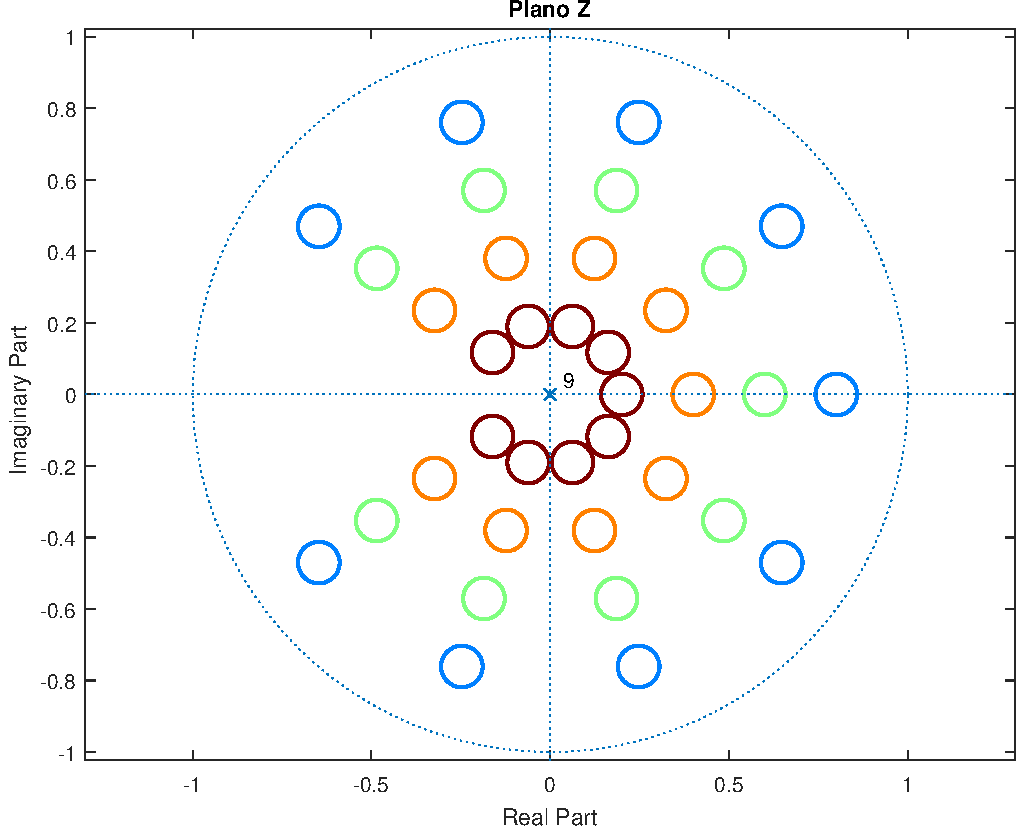
\includegraphics[width=\textwidth]{ex_3_pz_10}
	\end{subfigure}
	\begin{subfigure}{0.44\textwidth}
		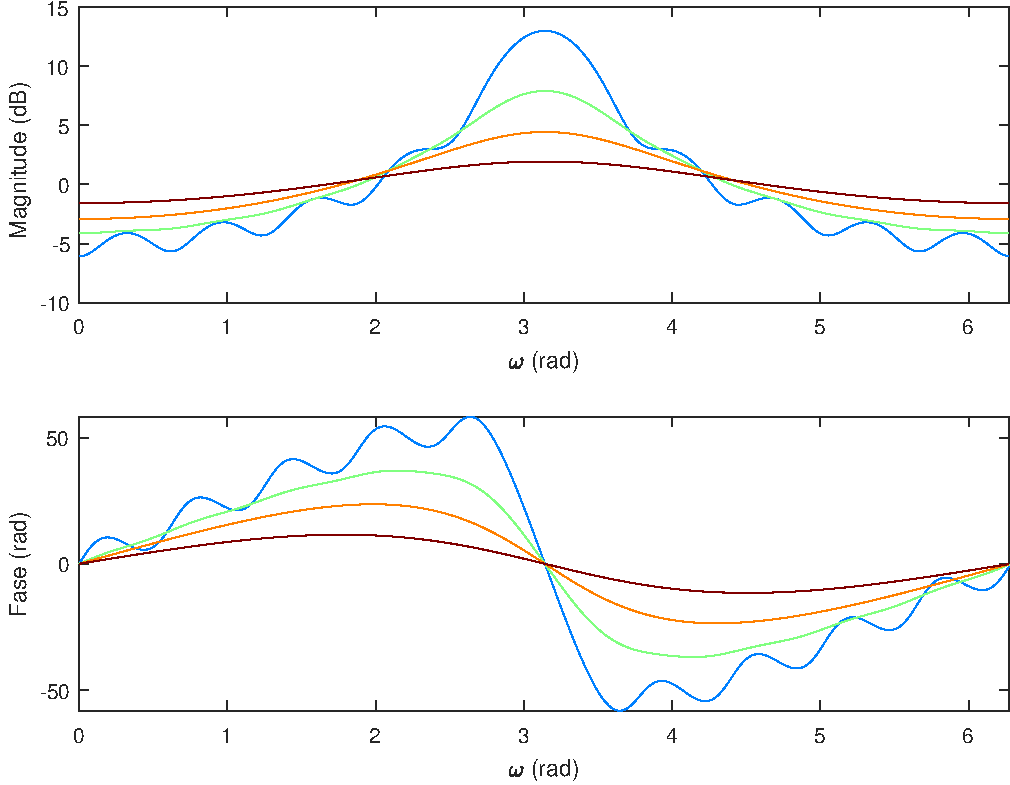
\includegraphics[width=\textwidth]{ex_3_bode_10}
	\end{subfigure}\\
		
	\caption{Visualizaç\~ao do Plano Z e das componentes de magnitude e fase para o sistema em \eqref{eq:second-system} com o par\^ametro $a < 0$}
	\label{fig:03}
\end{figure}

% ---------------------------------------------------------------
% End document
% ---------------------------------------------------------------

\end{document}

%%%%%%%%%%%%%%%%%%%%%%%%%%%%%%%%%%%
%% Drafts:
%%%%%%%%%%%%%%%%%%%%%%%%%%%%%%%%%%%
%%%%% Figure:
% \begin{figure}[ht]
%   \centering
%   \includegraphics[trim={0cm 0cm 0cm 0cm},clip,scale=1]{nameFigure}
%   \caption{Caption of the figure.}
%   \label{fig:nameFigure}
% \end{figure} \vskip0.25cm
%
%%%%% Equation:
% \begin{equation} \label{eq:nameEquation}
% \begin{split}
%    X = 1 + 1
% \end{split}
% \end{equation} \vskip0.25cm
%
%%%% Table:
% \begin{table}[hp]
%   \centering
%   \begin{tabular}{l | c c }
%   Principal & Coluna1 & Coluna2 \\
%   \hline 
%   ABC & 1 & 2 \\
%   DFG & 3 & 4 \\
%   HIJ & 5 & 6 \\
%   \end{tabular} 
%   \caption{Caption of the table.}
%   \label{table:nameTable} 
% \end{table} \vskip0.25cm

%\begin{figure}
%    \centering
%    \begin{minipage}[t][6cm][t]{.48\textwidth}
%	\begin{tikzpicture}
%	  \begin{axis}[enlargelimits=false, scale only axis, axis on top, width=0.8\textwidth,
%	  	xlabel={$u$ unemployment}, ylabel={$\pi$ inflation}]]
%		\addplot graphics [xmin=0,xmax=96,ymin=0,ymax=96] {chapter3/report_ch3_1_1};
%	  \end{axis}
%	 \end{tikzpicture}
%	\end{minipage}%
%	\hfill
%	\begin{minipage}[t][6cm][t]{0.48\textwidth}
%	\begin{tikzpicture}
%	  \begin{axis}[enlargelimits=false, scale only axis, axis on top, width=0.8\textwidth,
%	  	ylabel={$\pi$ inflation}]]
%		\addplot graphics [xmin=0,xmax=96,ymin=0,ymax=96] {chapter3/report_ch3_1_2};
%	  \end{axis}
%	\end{tikzpicture}%
%	\vspace{.6ex}
%	\begin{tikzpicture}
%		\begin{axis}[enlargelimits=false, scale only axis, axis on top, width=0.8\textwidth,
%	  	xlabel={$u$ unemployment}, ylabel={$\pi$ inflation}]]
%		\addplot graphics [xmin=0,xmax=96,ymin=0,ymax=96] {chapter3/report_ch3_1_3};
%		\end{axis}
%	\end{tikzpicture}
%	\end{minipage}%	
%    
%    \caption{A}
%    \label{fig:regulator01}
%\end{figure}